% ******************************************************************************%
%                                                                               % 
%         CDC_FancyCron.tex for FancyCron Project specification                 %
%            Made by: Eugène NGONTANG <ngonta_e@epitech.net>                    %
%                    engontan@bouyguestelecom.fr                                %
%                                                                               % 
% ******************************************************************************%

\documentclass{bouygues-fr}
%%\usepackage{sidecap}
\usepackage{supertabular}
\usepackage{longtable}

% ******************************************************************************%
%                                                                               % 
%                                 Prologue                                      %
%                                                                               % 
% ******************************************************************************%

\begin{document}



\title{\texttt{FancyCron}}
\subtitle{Cahier des charges Version 1.0.1}

\member{Eugène NGONTANG}{ngonta_e@epitech.net}
\member{DSI/DOQS/PFI Bougues Telecom}{engontan@bouyguestelecom.fr}

%%\newpage

\summary
{
  FancyCron est un logiciel de planification et d'exécution de tâches, pour système Linux et Windows. Le projet est né d'un besoin des administrateurs système de la DSI FAI de Bouygues Telecom.

  Ces derniers se servent du gestionnaire de tâches Linux Cron, pour l'automatisation des services réguliers sur l'ensemble des serveurs de leurs infrastructures.\\
  Ils se trouvent limités dans le suivi de ces tâches, sans informations pertinentes sur le déroulement de l'exécution des tâches de bout en bout.

  FancyCron viendra donc répondre à une problématique de planning production, de reporting et de gestion centralisée des tâches sur leurs environnements techniques. 

  Ce document constitue le cahier des charges destiné du projet, prenant en compte les besoins liés à sa réalisation et aux destinataires finaux(les administrateurs  système de la DSI FAI Bouygues  Telecom, et les utilisateurs du parc informatique).

  Il décrit également la manière dont l’équipe prendra en charge l’ensemble des phases du projet (analyse, conception, développement, documentation), les paramétrages, la reprise des données, et le support aux utilisateurs du logiciel.

  Nous  aborderons  dans  un  premier  temps  le  contexte  général  du  projet et  les  parties impliquées.

  Nous présenterons ensuite le projet, puis nous décrirons les prestations attendues de l’équipe de développement, et nous terminerons par les modalités de réalisation du projet.
}

\maketitle

\tableofcontents

\renewcommand{\labelitemi}{$\bullet$}
\renewcommand{\labelitemii}{$\circ$}

\newpage
% ******************************************************************************%
%                                                                               % 
%                                 Généralités                                   %
%                                                                               % 
% ******************************************************************************%
\chapter{Généralités}

\section{Contexte}

Dans l'optique d'augmenter sa productivité, tout en réduisant le temps de reprise de service après incident, l'équipe Socle FAI de la DSI Bouygues Telecom doit faire face à l'augmentation des coûts unitaires de l'ensemble de ses activités.

Une remise en cause profonde des méthodes de travail s'impose, parmi lesquelles l'automatisation des services réguliers.

En effet les administrateurs système du SI FAI disposent pour leurs environnements techniques, d'un nombre important de serveurs tournant principalement sous système Unix/Linux.

Le nombre d'applications et services installés sur ces serveurs est innombrable, et pour des contraintes techniques et contractuelles, ces services doivent être démarrés à des périodes précises, et fonctionner en permanence pour certains.

Cependant il serait pénible pour les ingénieurs système de procéder chaque fois au démarrage et à la mise en service manuels. D'où le besoin crucial d'un outil permettant le paramétrage et lancement automatique des taches.

Pour ce faire, les administrateurs systèmes du SI FAI Bouygues Telecom ont opté pour le logiciel Cron.

Cron est le nom d'un programme qui permet aux utilisateurs des systèmes Unix/Linux d'exécuter automatiquement des scripts ou des commandes à une date et une heure spécifiées, ou selon un cycle défini à l'avance.

C'est grâce à ce démon que se fait la gestion programmée et continue des services sur l'ensemble des serveurs du SI FAI Bouygues Telecom.

\vspace{20pt}

\section{La problématique}
Bien que l'utilisation des \textcolor{violet}{\texttt{« crontab »}} soit une pratique assez populaire et efficace pour l'exécution des tâches de fond, cette dernière peut s'avérer limitée dans certaines circonstances.

En effet:

\begin{itemize}
 \item l'utilisation des crontab nécessite un minimum de connaissances en administration système.
 \item avec cron, si le système est éteint au moment où la tâche a été planifiée, elle ne s'effectuera pas cette fois-ci. Il faudra attendre l'occurrence suivante pour voir la tâche s'executer.\\
Il n'est donc pas possible de rattraper des tâches avec cron, par exemple vérifier pour chaque tâche si elle a été lancée dans les \texttt{n} derniers jours, \texttt{n} étant la périodicité définie pour la tâche.

Ce qui est particulièrement gênant pour les administrateurs système du SI FAI de Bouygues Telecom. Ceux-ci se trouvent au moins une fois par semaine dans cette situation.
\item une autre difficulté de l'utilisation des crontab demeure dans la verbosité des fichiers de configuration, dans lesquels sont très souvent renseignés les chemins en dur des exécutables.\\
Nous pouvons également  noté la non granularité, voire l'absence d'informations sur la supervision des tâches planifiées.\\
Il n'existe aucun moyen prédéfini avec cron, de savoir à quel moment, et dans combien de temps doit s'exécuter une tâche. 
 \item par ailleurs, cron ne permet en rien de savoir si une tâche s'est terminée avec succès ou erreur, et le cas échéant de récupérer la sortie d'erreur générée.\\
C'est à l'administrateur d'user des moyens techniques dont il dispose, pour avoir toutes ces données. Ce qui peut s'avérer des fois approximatif et fastidieux.\\

Le fameux /dev/null vers lequel sont souvent redirigés les sorties des scripts exécutés par cron, n'est rien d'autre qu'un trash dont on ne peut voir le contenu.
 \end{itemize}

Ces quelques points suffisent pour justifier la nécessité d'optimiser la gestion des tâches de fond sur les serveurs du SI FAI.

\vspace{20pt}
\section{Le solutions existantes}
 En observant le problème d'un point de vue purement planification et gestion des tâches, nous avons fait une étude détaillée des solutions du marché, regroupés ici par type d'utilisation.

 Le but de cette section est surtout de permettre à l'équipe SI FAI de Bouygues Telecom d'avoir une vision globale des outils existant. Cela lui permet de filtrer ses besoins face à une offre importante de logiciels professionnels d’ordonnancement.
 \begin{figure}[H]
   %% \begin{center}
      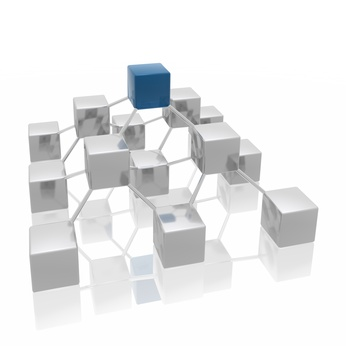
\includegraphics[width=5cm]{ordonnanceurs.jpg}
   %% \end{center}
  \end{figure}

  \begin{longtable}{| p{0.25\linewidth} | p{0.5\linewidth} | p{0.25\linewidth} |}
    %% \begin{tabularx}{15cm}{|c|p{4cm}|X|}
    \shrinkheight{-2cm}
    \hline
    \textcolor{violet}{\texttt{Rubrique}} & \textcolor{violet}{\texttt{Caractéristiques}} & \textcolor{violet}{\texttt{Logiciels}} \tabularnewline
    \hline
    Incontounables & 
    \begin{itemize}
    \item présents sur le marché français en terme de volume d’affaires et en représentation local (principalement en terme de support).
    \item représentent un intérêt dans un domaine particulier (production, open source, etc...)
    \item sont payant et proposent des versions d’évaluation
    \end{itemize} & 
    \textcolor{violet}{\texttt{Autosys, Control-M, Dollar Universe, OpCon™, Open source-job scheduler, Tivoli Workload Scheduler, Vega, Visual TOM, Workload Automation Autosys Edition}} \tabularnewline
    \hline
    Discrets &
    Apparaissent régulièrement dans les appels d’offre mais restent pourtant discrets sur au moins un des aspects suivants :
    \begin{itemize}
    \item pas assez diffusés et beaucoup trop peu de retour utilisateurs
    \item support en France sous-traité par une société tierce ou inextistant
    \item éditeur ne souhaitant pas communiquer les informations techniques sur le logiciel
    \end{itemize} &
    \textcolor{violet}{\texttt{APX, CA DSeries, Cronacle, JOB2DO, Ortro, TNG Workload, UC4}} \tabularnewline
    \hline
    Architectures distribuées &
    \begin{itemize}
    \item conçus pour exécuter des traitement sur des plateformes réparties/distribuées
    \item sont aussi sous licence payante
    \end{itemize} &
    \textcolor{violet}{\texttt{24x7 Automation Suite, ActiveBatch, Argent Job Scheduler, ASG-Zena, Automator, Avatar, Embarcadero Job Scheduler, Global ECS, JAMS, Open Process, OPSWise, PTC Scheduler, RoboIQ, Robot/Schedule, Saturn, Skybot, Tidal Enterprise, XS EnterpriseSchedule}} \tabularnewline
    \hline
    Services web &
    Prennent en compte les architectures J2EE &
    \textcolor{violet}{\texttt{24x7 Java edition, Essiembre Java Libraries, Flux, Fulcrum, Gos4J, OddJob}} \tabularnewline
    \hline
    Mainframes &
    \begin{itemize}
    \item premières machines à avoir fourni un système d’ordonnancement de tâches
    \item Certains ont été ensuite portés sur des machines plus petites pour être utilisés dans des architectures distribuées
    \end{itemize} &
    \textcolor{violet}{\texttt{BS2000 Job scheduling, CA-7, Zeke }} \tabularnewline
    \hline
    Orchestrateurs &
    &
    \textcolor{violet}{\texttt{ITPAM}} \tabularnewline
    \hline
    Planificateurs &
    Permettent de planifier une tâche mais ne peuvent être considérés comme des ordonnanceurs, car ils ne gèrent pas le séquencement &
    \textcolor{violet}{\texttt{Arcana Scheduler, AutoTask 2000, EZ Scheduler, FCron, Impact Scheduler, JCron, Macro Scheduler, PhpJobScheduler, PIKT, Schedule Wizard, SQL Scheduler, UNIJob / UNIViewer, Visual Cron}} \tabularnewline
    \hline
    Planificateurs système &
    Font partie intégrante du système d’exploitation &
    \textcolor{violet}{\texttt{Anacron, AT, DECScheduler}} \tabularnewline
    \hline
    Mono plateforme &
    Ne gèrent qu’un seul type de système d’exploitation, généralement Windows &
    \textcolor{violet}{\texttt{AdTempus, Automate, crondSys, LaunchPad, SmartBatch 2004}} \tabularnewline
    \hline
    Grid computing &
    Utilisent les ressources d’un ensemble de machines connectées comme on le ferait avec une seule machine. &
    \textcolor{violet}{\texttt{Condor, Dollar Universe NonStop Services, GridWay, JOSH, LSF, Maui Scheduler}} \tabularnewline
    \hline
    Composants de développement &
    Fournissent les fonctions de planification pour les développeurs et, éventuellement une interface.Mais cette dernière utilisation n’est pas sa vocation première &
    \textcolor{violet}{\texttt{Quartz, AutoFire, Avalon Task Scheduler, Enterprise Batch Server}} \tabularnewline
    \hline
    Queues batchs &
    Permet de soumettre des traitements qui seront régulés par une mécanisme de file d’attente &
    \textcolor{violet}{\texttt{GNU Queue, Java Batch Job Framework, jBatchEngine, JjobQ, Qed}} \tabularnewline
    \hline
    Intégrés &
    Intégrés dans le progiciel et ne peut être utilisé qu’à travers lui &
    \textcolor{violet}{\texttt{Cfengine, MySql, Oracle, SQL Server, Sybase, Sybercron}} \tabularnewline
    \hline
    Ateliers de production &
    \begin{itemize}
    \item dédiés aux ateliers de production 
    \item aucun vrai rapport avec les ordonnanceurs de tâches
    \item rubrique est purement informative
    \end{itemize}&
    \textcolor{violet}{\texttt{Quartis}} \tabularnewline
    \hline
    %% \end{tabularx}
  \end{longtable}

\vspace{18pt}
Nous pouvons remarquer que ces outils sont pour la plupart des ordonnanceurs, et disposent d'une gestion native des tâches.

Choisir un de ces logiciels à part ceux de la catégorie \texttt{Planificateurs systèmes}, serait mettre en place une nouvelle solution de gestion des tâches, qui ne s'intègre pas à la solution actuellement utilisée en interne.

Cela nécessite un retour arrière sur toute la solution actuellement déployée au socle SI FAI Bouygues Telecom.

Cron est la solution actuellement utilisée en interne, et fait partie des \texttt{Planificateurs systèmes}.

La problématique ne visant pas à remplacer \texttt{Cron}, mais à optimiser son utilisation, aucune des solutions que nous venons de citer ne répondrait au besoin.

\vspace{20pt}
\section{Le besoin}
L'équipe socle FAI de la DSI Bouygues Telecom désire avoir un outil qui sied le mieux aux méthodes de travail internes, aux procédures et contraintes de mise en production.

Cet outil doit s'intégrer et fonctionner avec \texttt{Cron}, sans le remplacer, mais l'alimenter en entrée et récupérer les informations générées en sortie.\\

Ainsi les principales fonctionnalités visées dans cette expression de besoin sont les suivantes :
\begin{itemize}
\item la possibilité d'activer/désactiver une crontab, et de savoir quels sont les tâches en cours d'exécution liées à la crontab
\item la possibilité de décaler l'exécution d'une crontab d'un certain temps (1h plus tôt ou tard), sans modifier le cycle normale d'exécution de la tâche (job)
\item pouvoir tracer l'exécution des scripts/services des crontab
\item connaître l'état de l'exécution des tâches (planning production)
\item visualiser l'état et les informations sur les crontab à travers une interface unifiée.\\
  Ces informations aideraient l'utilisateur par exemple pour le paramétrage, lors de la modification ou de la création d'une nouvelle crontab
\item pouvoir trier la liste des tâches par paramètre, en ordre croissant et décroissant. Exemple de paramètres de tri : Statut, Minute, Heure, Jour du mois, Mois, Jour de la semaine, Commande (chemin relatif ou absolu du binaire).
\item gérer les dépendances dans l'exécution des jobs : un script ne lance que si un autre s'est terminé, s'il s'est terminé avec succès ou s'il s'est terminé avec erreur
\end{itemize}

\newpage
  % ******************************************************************************%
  %                                                                               % 
  %                            Présentation du projet                             %
  %                                                                               % 
  % ******************************************************************************%
\chapter{Présentation du projet}

Pour faire face à la problématique ci-dessus, l'équipe  FAI de Bouygues Telecom a besoin d'un outil avec ces principales caractéristiques :
\begin{itemize}
\item facilité d'utilisation,
\item reporting sur l'exécution des tâches,
\item planning production.
\end{itemize}

\section{La solution à développer}
Le logiciel FancyCron n'est pas une reprise du projet Cron, il s'appuiera sur ce dernier en tant que surcouche et se composera de trois principaux modules :

\begin{itemize}
\item un module client \textcolor{violet}{\texttt{FancyCron-Client}}, en charge de l'exécution des tâches locales à chaque serveur en production. C'est ce module même qui va directement utiliser Cron.
\item un module d'administration \textcolor{violet}{\texttt{FancyCron-Admin}}, qui permettra l'administration et l'utilisation du logiciel à travers une interface web : création, modification des crontab, planification des tâches,...
\item un module monitoring \textcolor{violet}{\texttt{FancyCron-Monitor}}, qui surveillera l'état des tâches planifiées et remontera les informations à afficher. Il devra être paramétrable pour ne remonter que certaines informations.
\item un module serveur \textcolor{violet}{\texttt{FancyCron-Server}}, pour la gestion centralisée et le reporting des informations de crontab. C'est le seul module à avoir accès à tous les autres et auquel tous les autres ont accès. \\
  Il implémentera un patron lui permettant d'assurer ce rôle.
\item un module de notification \textcolor{violet}{\texttt{FancyCron-Notify}}, permettant l'envoi des notifications lorsqu'un évènement survient sur le système
\end{itemize}
 \begin{figure}[H]
    \begin{center}
      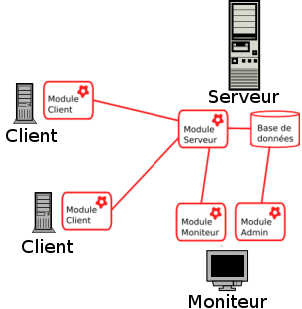
\includegraphics[width=6cm]{Architecture.png}
    \end{center}
    \caption{\scriptsize \texttt{Mode de fonctionnement FancyCron}}
  \end{figure}

\subsection{FancyCron-Client}
Ce module va se charger de toute la gestion des crontab sur le poste où il est installé.

Il encapsulera l'exécution des crontab dont il va gérer les entrées et sorties.

De ce fait les fichiers de configuration usuels des crontab sur les serveurs auront un format unifié, avec en paramètre commun un seul script utilisé par \textcolor{violet}{\texttt{FancyCron-Client}}. 

Désormais les seules différences visibles entre les lignes des fichiers de configuration de crontab seront principalement le cycle d'exécution de la crontab, et l'identifiant de la tâche à exécuter.

L'identifiant est une référence sur la commande à exécuter dans la crontab. 

\textcolor{violet}{\texttt{FancyCron-Client}} couvrira les fonctionnalités suivantes du logiciel :
\begin{itemize}
\item il utilisera un module de gestion de tâche qui implémentera un conteneur de tâches (\textcolor{violet}{\texttt{jobModule}}) instancié au démarrage du programme.
  
  Ce conteneur encapsulera pour chaque tâche spécifique, les paramètres suivants : 
  \begin{itemize}
  \item l'identifiant de tâche
  \item le nom de la tâche
  \item le staut de la tâche 
  \item le chemin de l'exécuatble ou la commande
  \item le cas échéant, les options tels ques reconnues par la commande, et les arguments de la commande
  \item la valeur de retour d'exécution de la tâche
  \item la durée d'exécution de la tâche
  \item Un paramètre permettant de stocker le calendrier sérialisé d'évènements de la tâche
  \item Un paramètre permettant de stocker l'historique d'exécution de la tâche(la valeur de rétention sera fixée pour la phase de développement)
\end{itemize}

Tous ces paramètres seront stockés en dur dans une base de données gérée par le serveur.
\\Il disposera donc des méthodes pour les récpérer au démarrage du programme, afin mettre à jour  le fichier de configuration crontab local. 

Il possèdera également un système de gestion d'erreurs pour ces fonctions.
\item le client FancyCron utilisera un module de gestion de dépendances (\textcolor{violet}{\texttt{jobDependenciesModule}}), définissant pour chaque tâche la liste des tâches dont elle dépend, avec le critère de dépendance associé.\\
  Ces informations seront stockées dans la même base que pour les paramètres cités plus haut.\\ Le \textcolor{violet}{\texttt{jobDependenciesModule}} permettra d'accéder à ces valeurs à l'exécution.
\item c'est au jobModule du client qu'incombe l'ordonnancement des tâches. Il devra s'occuper entre autres, de l'état d'une tâche : en cours, terminée, décalée,
 ok, ko, ....
\end{itemize}

FancyCron-Client communiquera directement avec FancyCron-Server.

\subsection{FancyCron-Admin}
FancyCron-Admin doit permettre aux utilisateurs du logiciel de créer des crontab via une interface web.

Ce module permet l'ajout d'une nouvelle tâche, la modification d'une tâche(renommer, décaler,...), avec des options de recherche sur les tâches.

L'admin FancyCron implémentera l'interface du logiciel, qui permettra à l'utilisateur d'accéder aux différentes fonctionnalités telles que :
\begin{itemize}
\item définir l'adresse email à laquelle les messages de crontab doivent être envoyés (logs, fichiers de sorties)
\item planifier de nouvelles tâches(crontab)
\item modifier des tâches
\item supprimer des tâches
\item activer, désactiver l'exécution d'une tâche (activer/désactiver la crontab)
\item décaler l'exécution d'une tâche d'une temps \textcolor{violet}{\texttt{t}} avant ou après l'heure d'exécution : le décalage prend en compte la période du cycle d'exécution que l'on souhaite décaler.

Il requiert également le temps de décalage à appliquer, ce qui permettra par exemple le rattrapage des exécutions manquées.
\end{itemize}

\subsection{FancyCron-Monitor}
FancyCron-Monitor permet de surveiller l'état des crontabs et affiche les informations dans l'interface utilisateur 

Ce module permettra de : 
\begin{itemize}
\item voir le statut des tâches (en cours, terminée, erreurs, ..). Cette visualisation doit se faire entre deux périodes consécutives du cycle d'exécution d'une tâche
\item lister les tâches retardées, en file d'attente (queue), en cours d'exécution, terminée. Ceci permettrait par exemple de diagnostiquer en cas d'incident
 \begin{figure}[H]
    \begin{center}
      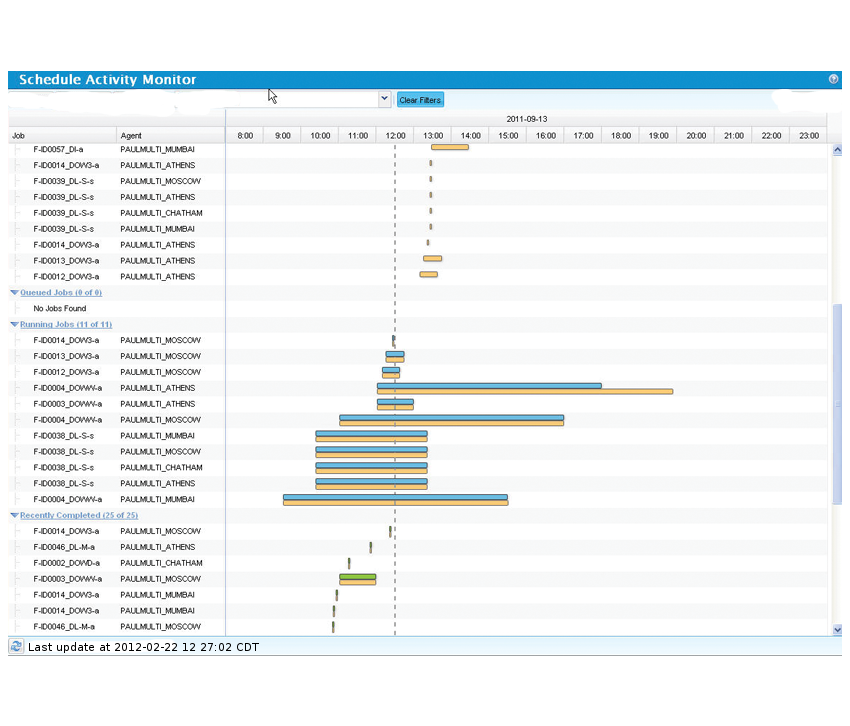
\includegraphics[width=10cm]{sam.png}
    \end{center}
    \caption{\scriptsize \texttt{Exemple d'affichage des tâches planifiées}}
  \end{figure}
\item le monitor doit afficher :
\begin{itemize}
\item l'heure prévu pour l'exécution de la tâche,
\item l'heure à la quelle la tâche a commencé,
\item le temps prévu pour l'exécution le cas échéant,
\item l'heure à la quelle elle s'est terminée
\end{itemize}
\item lister les tâches dont l'exécution n'a pas eu lieu, ou a eu lieu à une heure spécifiée, ainsi que les dépendances (tâches requises)
\item avoir un reporting sur l'exécution des tâches, grâce à un sous module de reporting utilisé dans ce module.\\
On pourra par exemple générer un rapport à l'aide d'un formulaire dans l'interface l'nterface utilisateur, suivant les critères proposés par le logiciel
\item voir les fichiers de sortie des commandes exécutées dans les crontab, sauvegarder les fichiers, les envoyer en pièces jointes, ou les supprimer
\item avoir un affichage trié des tâches, suivant les paramètres de tri mentionnés plus haut
\item avoir sur une page un historique des tâches, avec leurs états et les éventuels évènements qui se seraient produits lors de l'exécution d'une tâche
 \begin{figure}[H]
    \begin{center}
      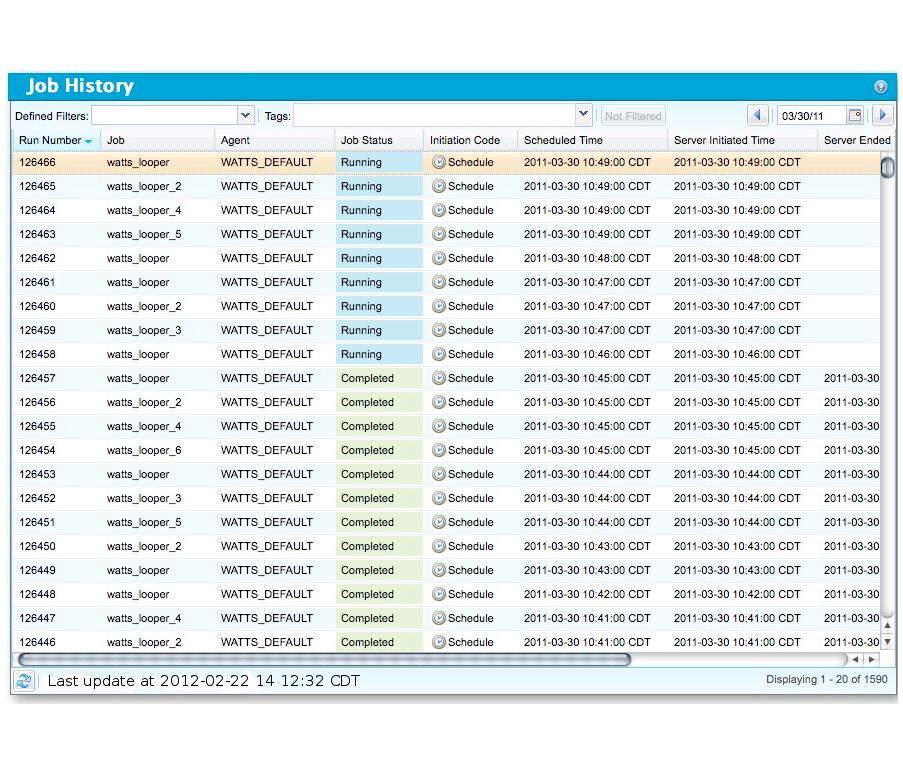
\includegraphics[width=10cm]{history.png}
    \end{center}
    \caption{\scriptsize \texttt{Historique des taches}}
  \end{figure}

\end{itemize}
Ce module sera développé en priorité avec l'IHM, pour juger et apprécier l'ergonomie du logiciel.

Toutes les considérations de développement seront consignées dans le document de conception et spécifications techniques.

Toutes les fonctionnalités du logiciel seront reportées sur l'IHM et exploitables par l'utilisateur via les modules Admin et Monitor

\subsection{FancyCron-Server}
Le module FancyCron-server  est au centre du fonctionnement du logiciel.

Non visible par les administrateurs et utilisateurs, il centralise les opérations de distribution et de collecte du système.

Ce module collecte les informations auprès des clients ou agents FancyCron et renvoie l’état des tâches au monitor.

Il aura  deux principaux  rôles : 
\begin{itemize}
\item la gestion centralisée des crontab 
\item le reporting des messages de crontab
\end{itemize}

 \begin{figure}[H]
    \begin{center}
      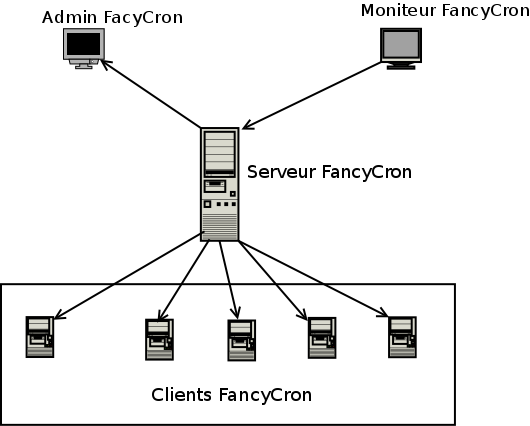
\includegraphics[width=10cm]{Interaction.png}
    \end{center}
    \caption{\scriptsize \texttt{Mode de communication FancyCron}}
  \end{figure}
Le module couvrira les caractéristiques suivantes :
\begin{itemize}
\item enregistrement des informations dans une base de données centralisée grâce à un module de stockage (\textcolor{violet}{\texttt{storageModule}}) qu'il embarque au démarrage.\\
  Le choix du système de gestion de base de données sera déterminé lors de la phase de conception.
\item transfert de paramètres de configuration au client, récupération des logs, résultats des commandes et autres messages de crontab du client.\\
  Il est clair que l'exécution des tâches est entièrement gérée en local par chaque client, et le serveur ne sert que distributeur(dispatcheur) pour la planification de ces tâches.
\item enregistrement/suppression des serveurs et groupe de serveurs utilisant les crontab
\item pour chaque utilisateur cron de chaque serveur, une liste des crontab associées
\item liste des tâches planifiées sur chaque serveur enregistré
\item liste et configuration des contacts pour messages crontab
\item gestion des dépendances non locales à un serveur (une tâche peut dépendre d'une autre non planifiée sur le même serveur)
\end{itemize}

\subsection{FancyCron-Notify}
Ce module permettra de paramétrer et de déclencher l'envoi des notifications, dans le système à mettre en oeuvre.

Il n'est pas obligatoire pour le fonctionnement de l'ensemble, les notifications pouvant être directement incluses au serveur.

Sa conception est donc entièrement laissée au soin du développeur.


\vspace{20pt}
\section{Contraintes}

\subsection{Environnement technique}

\begin{itemize}
\item La solution doit être portable, sous licence GPL, et fonctionner sur les systèmes Linux/UNIX et Windows, même si les premiers développements seront faits pour linux
\item Vue la modularité du système à développer, le choix d'un langage orienté objet s'impose.\\
Cependant le choix du langage doit aussi tenir compte de l'environnement de naissance du projet.

 Au SI FAI Bouygues Telecom, l'utilisation des langages interprétés est préconisé plutôt que les langages compilés.

Sur la base de ces deux contraintes, nous opterons pour le python qui est le mieux adapté à la situation,  de par sa conception objet et sa richesse en librairies.
\item La solution devra s'intégrer au logiciel Cron, et ne devra poser aucune contrainte à son utilisation de base.
\item Le logiciel devant s'utiliser via une interface web, un serveur web est requis.\\
Ainsi nous choisirons un des logiciels suivantes pour le serveur web : nginx(éventuellement couplé avec passenger), apache, cherrypy(éventuellement couplé à cheetah).

Le choix sera fait en tenant compte des contraintes matérielles du serveur web choisi, de la compatibilité avec python, et de l'évolution du logiciel développé.

Le choix du serveur web sera décidé lors de la phase de conception après analyse fonctionnelle.
\item Enfin un protocole sera défini pour la communication entre le client et le serveur FacncyCron
\end{itemize}

\subsection{Méthode de développement de la solution}

Le développement de la solution devra se faire de manière itérative et chaque itération à partir  de  la   deuxième,  devra  inclure  tous  les  modules.

Ci-dessous  une  proposition d’itérations :
\begin{itemize}
\item production d’une maquette IHM pour l’utilisateur final de la solution
\item mise en place d’un MCD (Modèle Conceptuel de Données)
\item conception de la solution :
  \begin{itemize}
  \item définition des données (toutes les informations nécessaires au développement des modules de la solution)
  \item Modélisation des traitements (un ou plusieurs diagrammes de séquences)
  \item Modélisation des objets nécessaires à la réalisation du projet (un ou plusieurs diagrammes de classes)
  \item Modélisation du processus interactif de l'ensemble du système (un ou plusieurs diagrammes d'activités)
  \end{itemize}
\item définition et documentation d'une API pour les plugins de l'application(un plugin devra inclure au moins une partie client, une partie serveur, une partie monitor ou une partie admin)
\item développement  des fonctionnalités IHM basiques :\\
  analyse, conception, développement, tests unitaires
\item développement d'un module Client de base (fonction d'historique des tâches locales en priorité) :\\
  analyse, conception, développement, tests unitaires
\item développement d'un module  Server de base (fonction de reporting en priorité) :\\
  analyse, conception, développement, tests unitaires
\item développement d'un module Admin de base :\\
  analyse, conception, développement, tests unitaires
\item développement d'un module Monitor de base :\\
  analyse, conception, développement, tests unitaires
\item production du premier prototype du logiciel(première version) incluant les fonctionnalités d'historique et de reporting des tâches :\\
  premiers assemblage, intégration et mise en production(Mise en Prod)
\item développement des fonctionnalités de tri et filtrage :\\
  analyse, conception, développement, tests unitaires
\item développement des fonctionnalités de gestion centralisée des crontabs et de planning production :\\
  analyse, conception, développement, tests unitaires
\item production du deuxième prototype du logiciel(deuxième version) incluant la gestion centralisée et planning production :\\
  assemblage, intégration et mise en production(Mise en Prod)
\item développement des fonctionnalités de gestion des dépendances :\\
  analyse, conception, développement, tests unitaires
\item production du troisième prototype du logiciel incluant l'ordonancement des tâches :\\
  assemblage, intégrations et mise en produtuction(Mise en Prod)
\item tests d’usines globaux et de vérification d’aptitude au bon fonctionnement (VABF)
\end{itemize}

\newpage
  % ******************************************************************************%
  %                                                                               % 
  %                              Prestation attendues                             %
  %                                                                               % 
  % ******************************************************************************%
\chapter{Prestation attendues}

\section {Approche}
Le  projet  FancyCron  est  découpé en trois phases ou parties (Cf voir shcéma cycle de dé développement ci-dessous).

\begin{itemize}
\item PHASE N\textdegree 1 : \textcolor{violet}{reporting et historisation des informations de crontab}
\item PHASE N\textdegree 2 : \textcolor{violet}{gestion centralisée et planning production}
\item PHASE N\textdegree 3 : \textcolor{violet}{ordonnancement et gestion des dépendances entre les tâches}
\end{itemize}


Chaque phase sera réalisée suivant un planning  détaillée et debouchera sur une version du logiciel.

La mise en oeuvre de chaque phase(version) s’appuira sur un découpage en lots.

Elle suivra une approche fonctionnelle et un cycle homogène, comme le montre la figure ci-dessous :

\begin{itemize}
\item LOT 1 : MODELISATION
\item LOT 2 : DEVELOPPEMENT
\item LOT 3 : HOMOLOGATION
\item LOT 4 : EXPLOITATION
\end{itemize}


La maîtrise d’ouvrage est réalisée par l'équipe du SI FAI de Bouygues Télécom.

\begin{itemize}
\item la modélisation
\item le développement(codage)
\item l'homologation
\item l'exploitation
\end{itemize}

 \begin{figure}[H]
    \begin{center}
      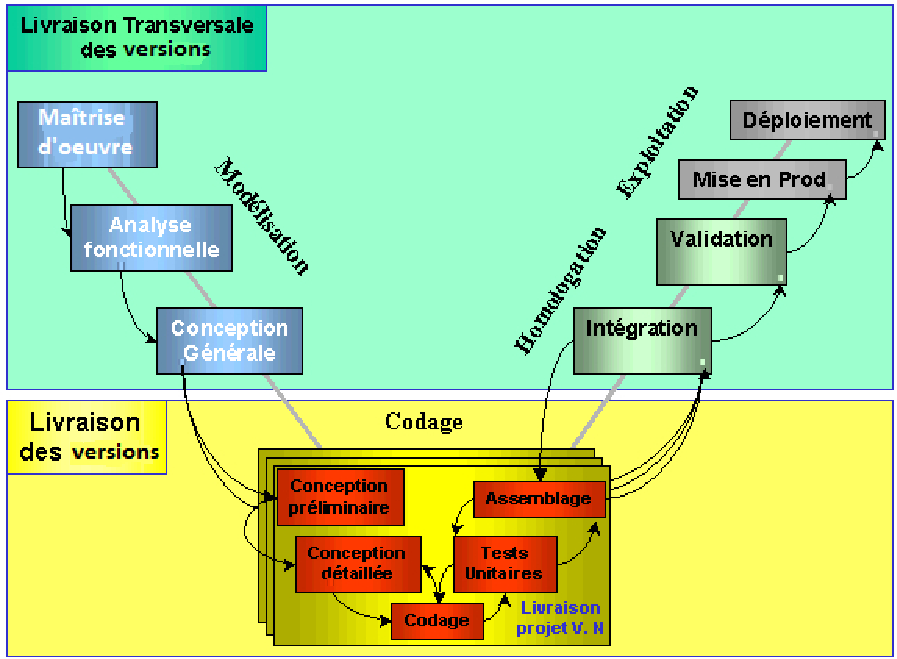
\includegraphics[width=10cm]{CycleDev.pdf}
    \end{center}
    \caption{\scriptsize \texttt{Cycle de développement du projet}}
  \end{figure}
  
Les flèches entre les différentes étapes de ce cycle de développement ilustrent les opération de promotion/rétrogadation au sein de la même version du logiciel, d'un ensemble de livrable : \texttt{code, spécifications textuelles, ressources diverses - images, fichiers de configuration, etc}.

\vspace{20pt}
\section{Modalités}

\subsection{Modalités de réalisation et livraison des prestations}
La mise en œuvre des prestations pour la première version du logiciel(PHASE N\textdegree 1) se fera suivant le planning suivant :
\begin{itemize}
\item \textcolor{violet}{Analyse fonctionnelle détaillée avant le 14/03/2012};
\item \textcolor{violet}{Spécifications avant le 22/03/2012};
\item \textcolor{violet}{Conception architecturale avant le 31/03/2012};
\item \textcolor{violet}{Conception détaillée avant le 07/04/2012};
\item \textcolor{violet}{Développement premier prototype avant le 31/05/2012};
\item \textcolor{violet}{Tests unitaires avant le 07/06/2012};
\item \textcolor{violet}{Tests d'intégration avant le 14/06/2012};
\item \textcolor{violet}{Tests de validation avant le 28/06/2012};
\item \textcolor{violet}{Formation et support avant le 05/07/2012};
\item \textcolor{violet}{Recette le 15/07/2012}.
\end{itemize}

Le planning ci-dessus correspond à 3 jours ouvrés par semaine consacrés au projet.

En tout état de cause, la vérification d’aptitude au bon fonctionnement pour la \\première version du logiciel doit être prononcée avant le 15/09/2012.

\subsection{Modalités de réception des prestations}
La réception des produits et services, sujets du présent projet fera l’objet d’une VABF (vérification d’aptitude au bon fonctionnement), et d’une VSR, (vérification de service régulier), par la maîtrise d'ouvrage.

La VABF est destinée à vérifier la conformité de l’ensemble des produits et services fournis par les développeurs, conformément aux stipulations du cahier des charges.

Dans l’hypothèse où la procédure de VABF donnerait lieu à d'éventuelles réserves, l'équipe projet devra procéder aux corrections   requises   et   à   la livraison d’une   nouvelle   version   des fournitures. Ceci dans des délais compatibles avec le calendrier.

\vspace{20pt}
\section {Gantt associé}
L'équipe projet établira un planning d’exécution des différentes phases du projet à remettre au SI FAI Bouygues Telecom.

Une proposition de planning des réalisations pour la première version du logiciel est consultable sur \href{https://mcp-d.admin.dolmen.bouyguestelecom.fr/fancycron/Planning/PlanningFancyCron.html}{ce lien}


  % ******************************************************************************%
\end{document}
